In this section, we have explored all the provided datasets to understand their properties, size and scale. We have also performed analysis of how these datasets correlate with the provided problem.

\subsubsection{What are the different properties, size and scale of data?}

After importing all the provided datasets using \texttt{pandas} python package, we deduced following summary of the data for the categorical variables:

\begin{itemize}
    \item Space metadata(\texttt{uom-space}) contains data of \texttt{7 campuses} which comprises of \texttt{331 buildings}. These buildings have \texttt{28 floor codes} and total \texttt{5703 rooms} which belongs to \texttt{185 room types}. 
    \item This metadata can be enhanced with \texttt{rm-category-type} dataset which contains room information of \texttt{209 different room types}.
    \item This metadata can also be enhanced with \texttt{fl-name} dataset which contains floor information of all possible floor codes.
    \item Audio-visual equipment dataset contains data of  \texttt{1964 equipments} which belongs to \texttt{32 manufacturers}. These equipments can be found in \texttt{11 campuses} across \texttt{142 buildings}.
    \item Employee dataset contains location information of \texttt{7709 employees} who are located across \texttt{130 buildings} and \texttt{1565 room codes}.
    \item Timetable data contains information for \texttt{52 departments} that have classes for \texttt{1577 modules} which occurs across \texttt{248 activity dates} throughout the year.
    \item Meeting room usage dataset contains information of meetings held throughout the year in \texttt{890 meeting rooms} across \texttt{8 campuses} and \texttt{125 buildings}.
\end{itemize}

Similarly, we deduced summary of the important numerical variables provided in the datasets:

\begin{itemize}
    \item Space metadata contains variable \texttt{Room Capacity} which ranges from \texttt{0-599} with an average of \texttt{4.0627} and standard deviation of \texttt{17.2592}.
    \item Space metadata also contains \texttt{Room Area $m^2$} which ranges from \texttt{0.22-5696.90} with an average of \texttt{30.70} and standard deviation of \texttt{118.3070}.
    \item Timetable dataset contains \texttt{Planned Size} which gives possible students that can attend a particular class. This variable ranges from \texttt{0-684} with average of \texttt{50 students}.
    \item Timetable dataset also provides \texttt{Class Duration (min)} which ranges from \texttt{30-675} with an average of \texttt{94.336}.
    \item Meeting rooms usage dataset contains \texttt{Meetings} parameter which gives a count of number of meetings held throughout the year. It ranges from \texttt{0-1000} with an average of \texttt{241 meetings}.
\end{itemize}

\subsubsection{How is the data distributed across features?}

In our analysis, we explored different categorical and numerical features of the datasets to get more depth about the data. Initially, we saw that most of the data is provided for the \texttt{Parkville} campus as shown in the Figure \ref{fig:expo-image-1}. Due to this huge skewness, we have performed our data and correlation analysis on the parkville campus in this report, which can be easily extended to other campuses in the future phase of this project.

\begin{figure}[H]
\centering
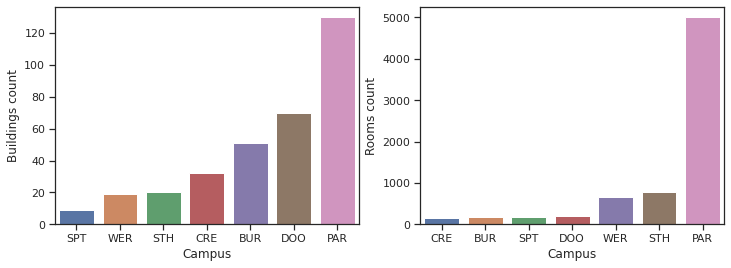
\includegraphics[width=12cm,keepaspectratio=true]{snap-1}
\caption{Distribution of buildings and rooms across campus}
\label{fig:expo-image-1}
\end{figure}

So, we explored different covariates provided in the space metadata and analysed them for the parkville campus. We saw that most of the buildings have rooms with \texttt{stair} or \texttt{circulation} as their room types. Most of the rooms are found at \texttt{Level 1, Ground or Level 2} floors across all provided buildings. Similarly, we found that \texttt{conf/meeting} room types have the highest total room capacity of around 6000 students and \texttt{circ-department} room type has the highest combined room area in $m^2$. We also saw that most of the rooms are in \texttt{Excellent} and \texttt{Good} room conditions where highest number of rooms belonged to \texttt{UNIGEN} department.

Using room category data and merging it with space metadata, we were able to figure out the distribution of meeting rooms and toilet facilities across buildings in the Parkville campus as shown in Figure \ref{fig:expo-image-2}. We saw that \texttt{333 Exhibition st} building has the highest number of meeting rooms and \texttt{The spot} building has the highest number of toilet facilities.

\begin{figure}[H]
\centering
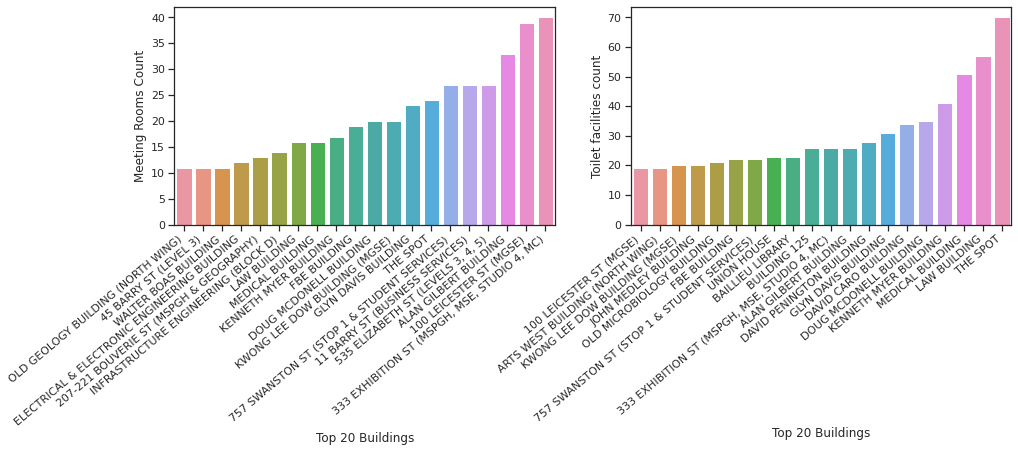
\includegraphics[width=16cm,keepaspectratio=true]{snap-2}
\caption{Distribution of meeting rooms and toilet facilities across buildings}
\label{fig:expo-image-2}
\end{figure}

We did the same analysis on the employee data for the parkville campus and saw that most of the staff members are located in \texttt{Doug Mcdonell Building} followed by \texttt{Business Services} building. They usually sit in the room which has \texttt{shared prostaff} or \texttt{shared grades} as their room types. Moreover, they are mostly located on the \texttt{Level 3} across buildings and mostly belong to the department \texttt{4140}.

Similarly, analysis of audio visual equipment dataset reveals that most of the equipments are of \texttt{Fuji Xerox} manufacturer with \texttt{Print staff} as their equipment standard. Most of the meeting rooms with equipments are found in \texttt{Kwong Lee Dow building} and they are usually located on \texttt{Level 1} across buildings.

Finally, we did the same analysis on the timetable data and meeting room usage data. We saw that most of the classes are scheduled for \texttt{MDHS} department where \texttt{MGSE} department has the highest number of modules. Similarly, we saw that most of the meetings are being held at \texttt{Stop 1} building followed by \texttt{Alan gilbert} building where 84\% of these rooms are in \texttt{Excellent} condition.

\subsubsection{How is the data connected with the problem?}

After exploring different properties and aspects of the data, we tried to see and understand how data can be used to get the basic intuition of the problem.

In order to do that, we created several supply-demand plots across various covariates which helped to see the need of space optimization. Initially, we created supply-demand plots based on the very trivial preference of staff members trying to book a meeting room in the same building where they are located. This plot is shown in the Figure \ref{fig:expo-image-3}. As per the plot, we can clearly see space optimization problem in terms of supply and demand proportion especially in the \texttt{Law Building}, \texttt{Doug Mcdonell building} and \texttt{Kenneth Myer building}.

\begin{figure}[H]
\centering
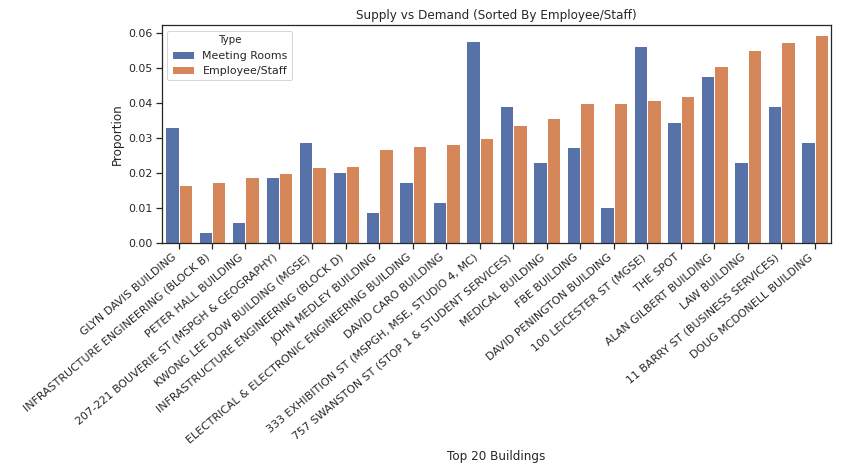
\includegraphics[width=10cm,keepaspectratio=true]{snap-3}
\caption{Supply vs Demand of meeting rooms across buildings}
\label{fig:expo-image-3}
\end{figure}

 Similarly, we created supply-demand plot on the same trivial preference of students trying to access a toilet facility in the same building which is shown in the Figure \ref{fig:expo-image-4}. Again, we can see that space optimization problem in terms of supply and demand proportion especially for \texttt{Redmond barry building}.
 
\begin{figure}[H]
\centering
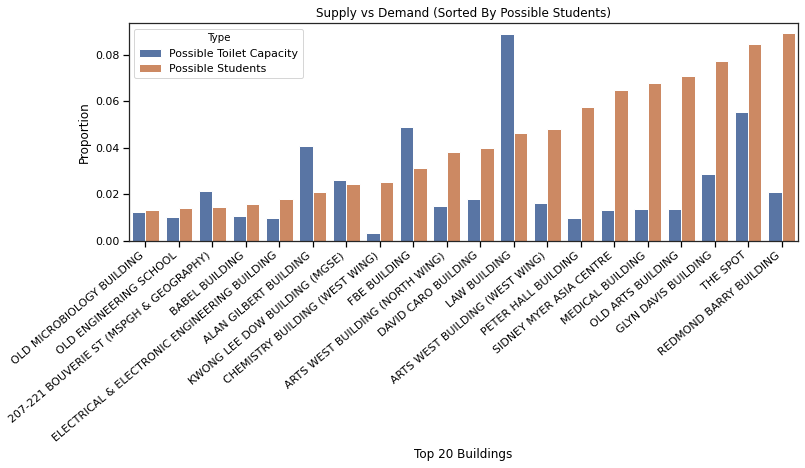
\includegraphics[width=10cm,keepaspectratio=true]{snap-4}
\caption{Supply vs Demand of toilet facilities across buildings}
\label{fig:expo-image-4}
\end{figure}

We have explored several other covariates with respect to supply-demand in Section \ref{correlations} which will eventually help us to perform space optimization on the underlying problem.